\documentclass{article}

\usepackage{graphicx}
\usepackage{amsmath,amssymb}
\usepackage[none]{hyphenat}
\usepackage{cite}
\usepackage{hyperref}

\title{Discrete Codes for Extreme Embedding Compression in Retrieval Systems}
\author{Guillermo Pasquero}

\begin{document}

\maketitle

\begin{abstract}
Modern embedding systems rely on dense floating-point vectors as the default representation for semantic similarity and retrieval tasks. However, under tight memory constraints, such representations may be suboptimal.

In this work, we investigate extreme embedding compression and show that discrete representations based on residual vector quantization (RVQ) can outperform dense PCA-based compression in low-memory regimes. We propose SERA-VQ, a simple pipeline combining PCA dimensionality reduction with residual vector quantization, encoding each embedding as a short sequence of discrete codes.

Across both semantic similarity (STS-B) and retrieval benchmarks (BEIR SciFact), we find a consistent pattern: while dense PCA with quantization remains competitive at moderate to high memory budgets, discrete codes significantly outperform dense embeddings when the memory per vector is constrained to 32 bytes or less. In particular, at 32 bytes per embedding, SERA-VQ achieves a substantial improvement in retrieval quality (nDCG@10: 0.560 vs. 0.451) compared to PCA with int8 quantization.

These results reveal a previously underexplored regime where dense vector representations are no longer optimal, and suggest that discrete codes provide a more efficient alternative for memory-constrained retrieval systems.
\end{abstract}

\section{Introduction}

Dense vector embeddings have become the dominant representation for semantic similarity and information retrieval tasks. Modern systems rely on high-dimensional continuous vectors, typically learned via neural encoders, and operate using similarity measures such as cosine similarity. This paradigm has proven highly effective across a wide range of applications, including search, recommendation, and natural language understanding.

However, the widespread adoption of embedding-based systems has introduced new constraints, particularly in large-scale and memory-limited settings. Storing and processing dense floating-point vectors can become prohibitively expensive, especially when dealing with millions or billions of embeddings. As a result, a substantial body of work has focused on compressing embeddings through techniques such as dimensionality reduction, quantization, and approximate nearest neighbor search.

Among these approaches, principal component analysis (PCA) combined with low-precision quantization (e.g., int8) represents a strong and widely used baseline. PCA provides an optimal linear projection in terms of variance preservation, while quantization reduces storage costs with minimal impact on similarity metrics. In practice, this combination offers an effective trade-off between compression and performance across many tasks.

In this work, we revisit the problem of embedding compression under extreme memory constraints and challenge the implicit assumption that dense vector representations remain optimal in this regime. We ask a simple but fundamental question: are dense embeddings still the best representation when each vector must be compressed to only a few dozen bytes?

To answer this, we investigate discrete representations based on residual vector quantization (RVQ). We introduce SERA-VQ, a simple pipeline that first applies PCA for dimensionality reduction and then encodes embeddings as short sequences of discrete codebook indices. This results in highly compact representations, where each embedding can be stored in as little as 8--32 bytes.

Our empirical results reveal a clear and consistent pattern across both semantic similarity (STS-B) and retrieval benchmarks (BEIR SciFact). While dense PCA-based compression remains competitive at moderate to high memory budgets, discrete representations significantly outperform dense embeddings in the low-memory regime. In particular, at 32 bytes per embedding, SERA-VQ achieves substantial gains in retrieval quality compared to PCA with int8 quantization.

These findings highlight the existence of a previously underexplored regime in which dense embeddings are no longer optimal, and suggest that discrete codes provide a more effective representation under tight memory constraints. This challenges the prevailing assumption that continuous vector spaces are inherently superior, and opens the door to alternative representations for large-scale retrieval systems.

In summary, the contributions of this work are as follows:
\begin{itemize}
    \item We demonstrate that dense PCA-based compression becomes suboptimal under extreme memory constraints.
    \item We propose SERA-VQ, a simple and effective discrete representation based on residual vector quantization.
    \item We provide empirical evidence across semantic similarity and retrieval benchmarks showing that discrete codes outperform dense embeddings in low-memory regimes.
\end{itemize}

\section{Related Work}

Embedding compression has been extensively studied in the context of large-scale retrieval and similarity search. Existing approaches can be broadly categorized into dimensionality reduction, quantization, and discrete representation methods.

\paragraph{Dimensionality reduction.}
Principal component analysis (PCA)~\cite{pca} is one of the most widely used techniques for compressing embeddings. By projecting vectors onto a lower-dimensional subspace that maximizes variance, PCA provides an optimal linear compression under mean squared error. In practice, PCA is often combined with low-precision representations such as int8 to further reduce memory usage while preserving similarity structure.

\paragraph{Quantization methods.}
Vector quantization techniques, including product quantization (PQ)~\cite{pq} and its variants, have been widely adopted for efficient nearest neighbor search. These methods partition the vector space into subspaces and quantize each independently, enabling compact representations and fast distance computation. Residual vector quantization (RVQ) extends this idea by iteratively quantizing the residual error, providing higher fidelity approximations at the cost of additional codebooks.

\paragraph{Discrete representations.}
More recent work has explored fully discrete or symbolic representations of embeddings, motivated by efficiency and robustness considerations. These approaches aim to replace continuous vectors with compact codes, often learned through clustering, hashing, or neural quantization techniques. While such methods have shown promise, their performance relative to strong baselines such as PCA with quantization remains insufficiently explored, particularly under extreme compression constraints.

\paragraph{Sentence embeddings and retrieval benchmarks.}
Sentence-Transformers~\cite{sbert} have become a standard for producing dense semantic representations of text, while BEIR~\cite{beir} provides a heterogeneous benchmark suite for the zero-shot evaluation of information retrieval models. We rely on both in our experimental setup.

\paragraph{Our contribution.}
In contrast to prior work, we focus explicitly on the low-memory regime, where embeddings must be compressed to a few dozen bytes or less. We show that in this setting, standard dense representations become suboptimal, and that simple discrete codes based on residual vector quantization can outperform PCA-based compression. Our results highlight a regime that has received limited attention and suggest a shift in representation choice under tight memory constraints.

\section{Method}

We propose SERA-VQ, a simple pipeline for compressing dense embeddings into compact discrete representations. The method combines linear dimensionality reduction with residual vector quantization, producing a sequence of discrete codes for each embedding.

\subsection{Overview}

Given an input embedding $x \in \mathbb{R}^d$, SERA-VQ applies two steps:

\begin{enumerate}
    \item Dimensionality reduction via PCA
    \item Residual vector quantization (RVQ)
\end{enumerate}

The final representation is a sequence of discrete indices corresponding to codebook entries, requiring only a few bytes per embedding.

\subsection{PCA Projection}

We first reduce the dimensionality of the input embedding using principal component analysis. Let $P \in \mathbb{R}^{k \times d}$ be the PCA projection matrix. The reduced embedding is:

\[
z = P x
\]

where $z \in \mathbb{R}^k$ and $k \ll d$.

This step preserves most of the variance of the original embedding while significantly reducing dimensionality.

\subsection{Residual Vector Quantization}

We then apply residual vector quantization to the reduced embedding $z$.

RVQ represents a vector as a sum of codewords selected from a sequence of codebooks:

\[
z \approx \sum_{i=1}^{M} c_i
\]

where each $c_i$ is selected from a codebook $\mathcal{C}_i$ of size $K$.

The encoding proceeds iteratively:

\begin{enumerate}
    \item Initialize residual $r_0 = z$
    \item For $i = 1, \dots, M$:
    \begin{itemize}
        \item Select codeword $c_i \in \mathcal{C}_i$ minimizing $\|r_{i-1} - c_i\|^2$
        \item Update residual $r_i = r_{i-1} - c_i$
    \end{itemize}
\end{enumerate}

Each codeword is represented by its index, resulting in a compact discrete representation:

\[
\text{code}(z) = (i_1, i_2, \dots, i_M)
\]

where each index $i_j \in \{1, \dots, K\}$.

In our implementation, we use $K = 256$ centroids per codebook, allowing each index to be stored in a single byte.

\subsection{Storage and Compression}

The total memory per embedding is $M$ bytes, where $M$ is the number of codebooks.

For example:

\begin{itemize}
    \item $M = 32$ $\Rightarrow$ 32 bytes per embedding
    \item $M = 16$ $\Rightarrow$ 16 bytes per embedding
\end{itemize}

Compared to the original float32 representation (e.g., 1536 bytes), this results in compression ratios of up to 48$\times$--192$\times$.

\subsection{Similarity Computation}

To evaluate similarity, we reconstruct approximate embeddings:

\[
\hat{z} = \sum_{i=1}^{M} c_i
\]

and compute cosine similarity between reconstructed vectors.

While more efficient distance computations are possible using lookup tables, we use reconstruction-based similarity for simplicity and consistency with dense baselines.

\subsection{Discussion}

SERA-VQ introduces a non-linear representation through the use of discrete codebooks, in contrast to purely linear compression methods such as PCA. This allows it to better preserve local structure in the embedding space under extreme compression, which we hypothesize contributes to its improved performance in low-memory regimes.

\section{Experiments}

We evaluate SERA-VQ on both semantic similarity and retrieval tasks, focusing on the low-memory regime. Our goal is to compare discrete representations against strong dense baselines under strict memory constraints.

\subsection{Datasets}

We consider two complementary benchmarks:

\paragraph{STS-B.}
The Semantic Textual Similarity Benchmark (STS-B) evaluates the ability of embeddings to capture semantic similarity between sentence pairs. Performance is measured using Spearman correlation between predicted similarities and human judgments.

\paragraph{BEIR SciFact.}
We use the SciFact dataset from the BEIR benchmark to evaluate retrieval performance. SciFact consists of scientific claims paired with relevant supporting documents. We report standard retrieval metrics, including Recall@10 and nDCG@10.

\subsection{Embedding Model}

All experiments use the \texttt{all-MiniLM-L6-v2} model from the Sentence-Transformers library. This model produces 384-dimensional embeddings, which serve as the input to all compression methods.

\subsection{Baselines}

We compare SERA-VQ against strong dense compression baselines:

\paragraph{PCA + float32.}
Embeddings are projected to a lower-dimensional space using PCA and stored in float32 format.

\paragraph{PCA + int8.}
Embeddings are projected using PCA and quantized to 8-bit integers, representing a widely used compression baseline.

We evaluate multiple dimensionalities (e.g., 32, 64, 96, 128) to explore the trade-off between memory and performance.

\subsection{SERA-VQ Configuration}

For SERA-VQ, we apply PCA followed by residual vector quantization. We vary:

\begin{itemize}
    \item PCA dimensionality ($k$)
    \item Number of codebooks ($M$)
\end{itemize}

Each codebook contains 256 centroids, allowing each code to be stored in one byte. As a result, the total memory per embedding is equal to the number of codebooks.

We evaluate configurations corresponding to 8, 16, 24, and 32 bytes per embedding.

\subsection{Evaluation Protocol}

For STS-B, we compute cosine similarity between reconstructed embeddings and report Spearman correlation.

For BEIR SciFact, we perform brute-force retrieval using cosine similarity and report Recall@10 and nDCG@10.

All embeddings are normalized prior to similarity computation. For discrete representations, we reconstruct approximate embeddings before evaluation to ensure consistency with dense baselines.

\subsection{Implementation Details}

PCA is trained on the training split of the dataset. Residual vector quantization is implemented using MiniBatch K-Means for each codebook, trained sequentially on residuals.

All experiments are conducted using standard Python libraries, including \texttt{sentence-transformers}, \texttt{scikit-learn}, and \texttt{numpy}. The full implementation is available in the accompanying repository.

The full implementation, experimental scripts, and reproducible pipelines are available at:
\url{https://github.com/gpasquero/sera-vq}.

\section{Results}

\subsection{Semantic Similarity (STS-B)}

We first evaluate performance on the STS-B benchmark, focusing on the relationship between memory usage and semantic similarity.

Figure~\ref{fig:sts} shows the trade-off between memory per embedding and Spearman correlation. At moderate to high memory budgets (e.g., 64 bytes and above), PCA with int8 quantization remains highly competitive and often achieves the best performance.

However, a different pattern emerges in the low-memory regime. When the memory per embedding is constrained to 32 bytes or less, discrete representations based on SERA-VQ outperform dense PCA-based compression. In particular, at 32 bytes, SERA-VQ achieves higher correlation than PCA with int8 quantization, despite using the same memory budget.

These results suggest that linear compression methods such as PCA become suboptimal under extreme compression, while discrete codes better preserve semantic structure in this regime.

\subsection{Retrieval Performance (BEIR SciFact)}

We next evaluate retrieval performance on the BEIR SciFact benchmark, using nDCG@10 and Recall@10 as metrics.

Figure~\ref{fig:beir} presents the trade-off between memory and retrieval quality. The results show a clear advantage for discrete representations in the low-memory regime.

At 32 bytes per embedding, SERA-VQ achieves a substantial improvement over PCA with int8 quantization:

\begin{itemize}
    \item PCA + int8 (32 bytes): nDCG@10 = 0.451
    \item SERA-VQ (32 bytes): nDCG@10 = 0.560
\end{itemize}

This corresponds to a large relative improvement in ranking quality, while maintaining the same memory footprint.

Interestingly, SERA-VQ at 32 bytes also matches or exceeds the performance of PCA at higher memory budgets. For example, SERA-VQ (32 bytes) achieves comparable performance to PCA with 64 bytes, highlighting the efficiency of discrete representations.

\subsection{Memory--Performance Trade-off}

Across both STS-B and BEIR, we observe a consistent pattern:

\begin{itemize}
    \item At high memory budgets, dense PCA-based compression remains strong.
    \item At low memory budgets ($\leq$32 bytes), discrete representations outperform dense embeddings.
\end{itemize}

This indicates the presence of a regime shift in which the optimal representation changes as memory constraints become more severe.

Figure~\ref{fig:sts} and Figure~\ref{fig:beir} illustrate this transition, with a clear crossover point around 32 bytes per embedding.

\subsection{Discussion}

The observed improvements suggest that discrete representations introduce beneficial non-linear structure that is not captured by linear methods such as PCA. Under extreme compression, this allows SERA-VQ to better preserve local relationships in the embedding space, which are critical for both similarity and retrieval tasks.

Overall, our results demonstrate that discrete codes provide a more effective representation than dense embeddings in memory-constrained settings.

\begin{figure}[t]
    \centering
    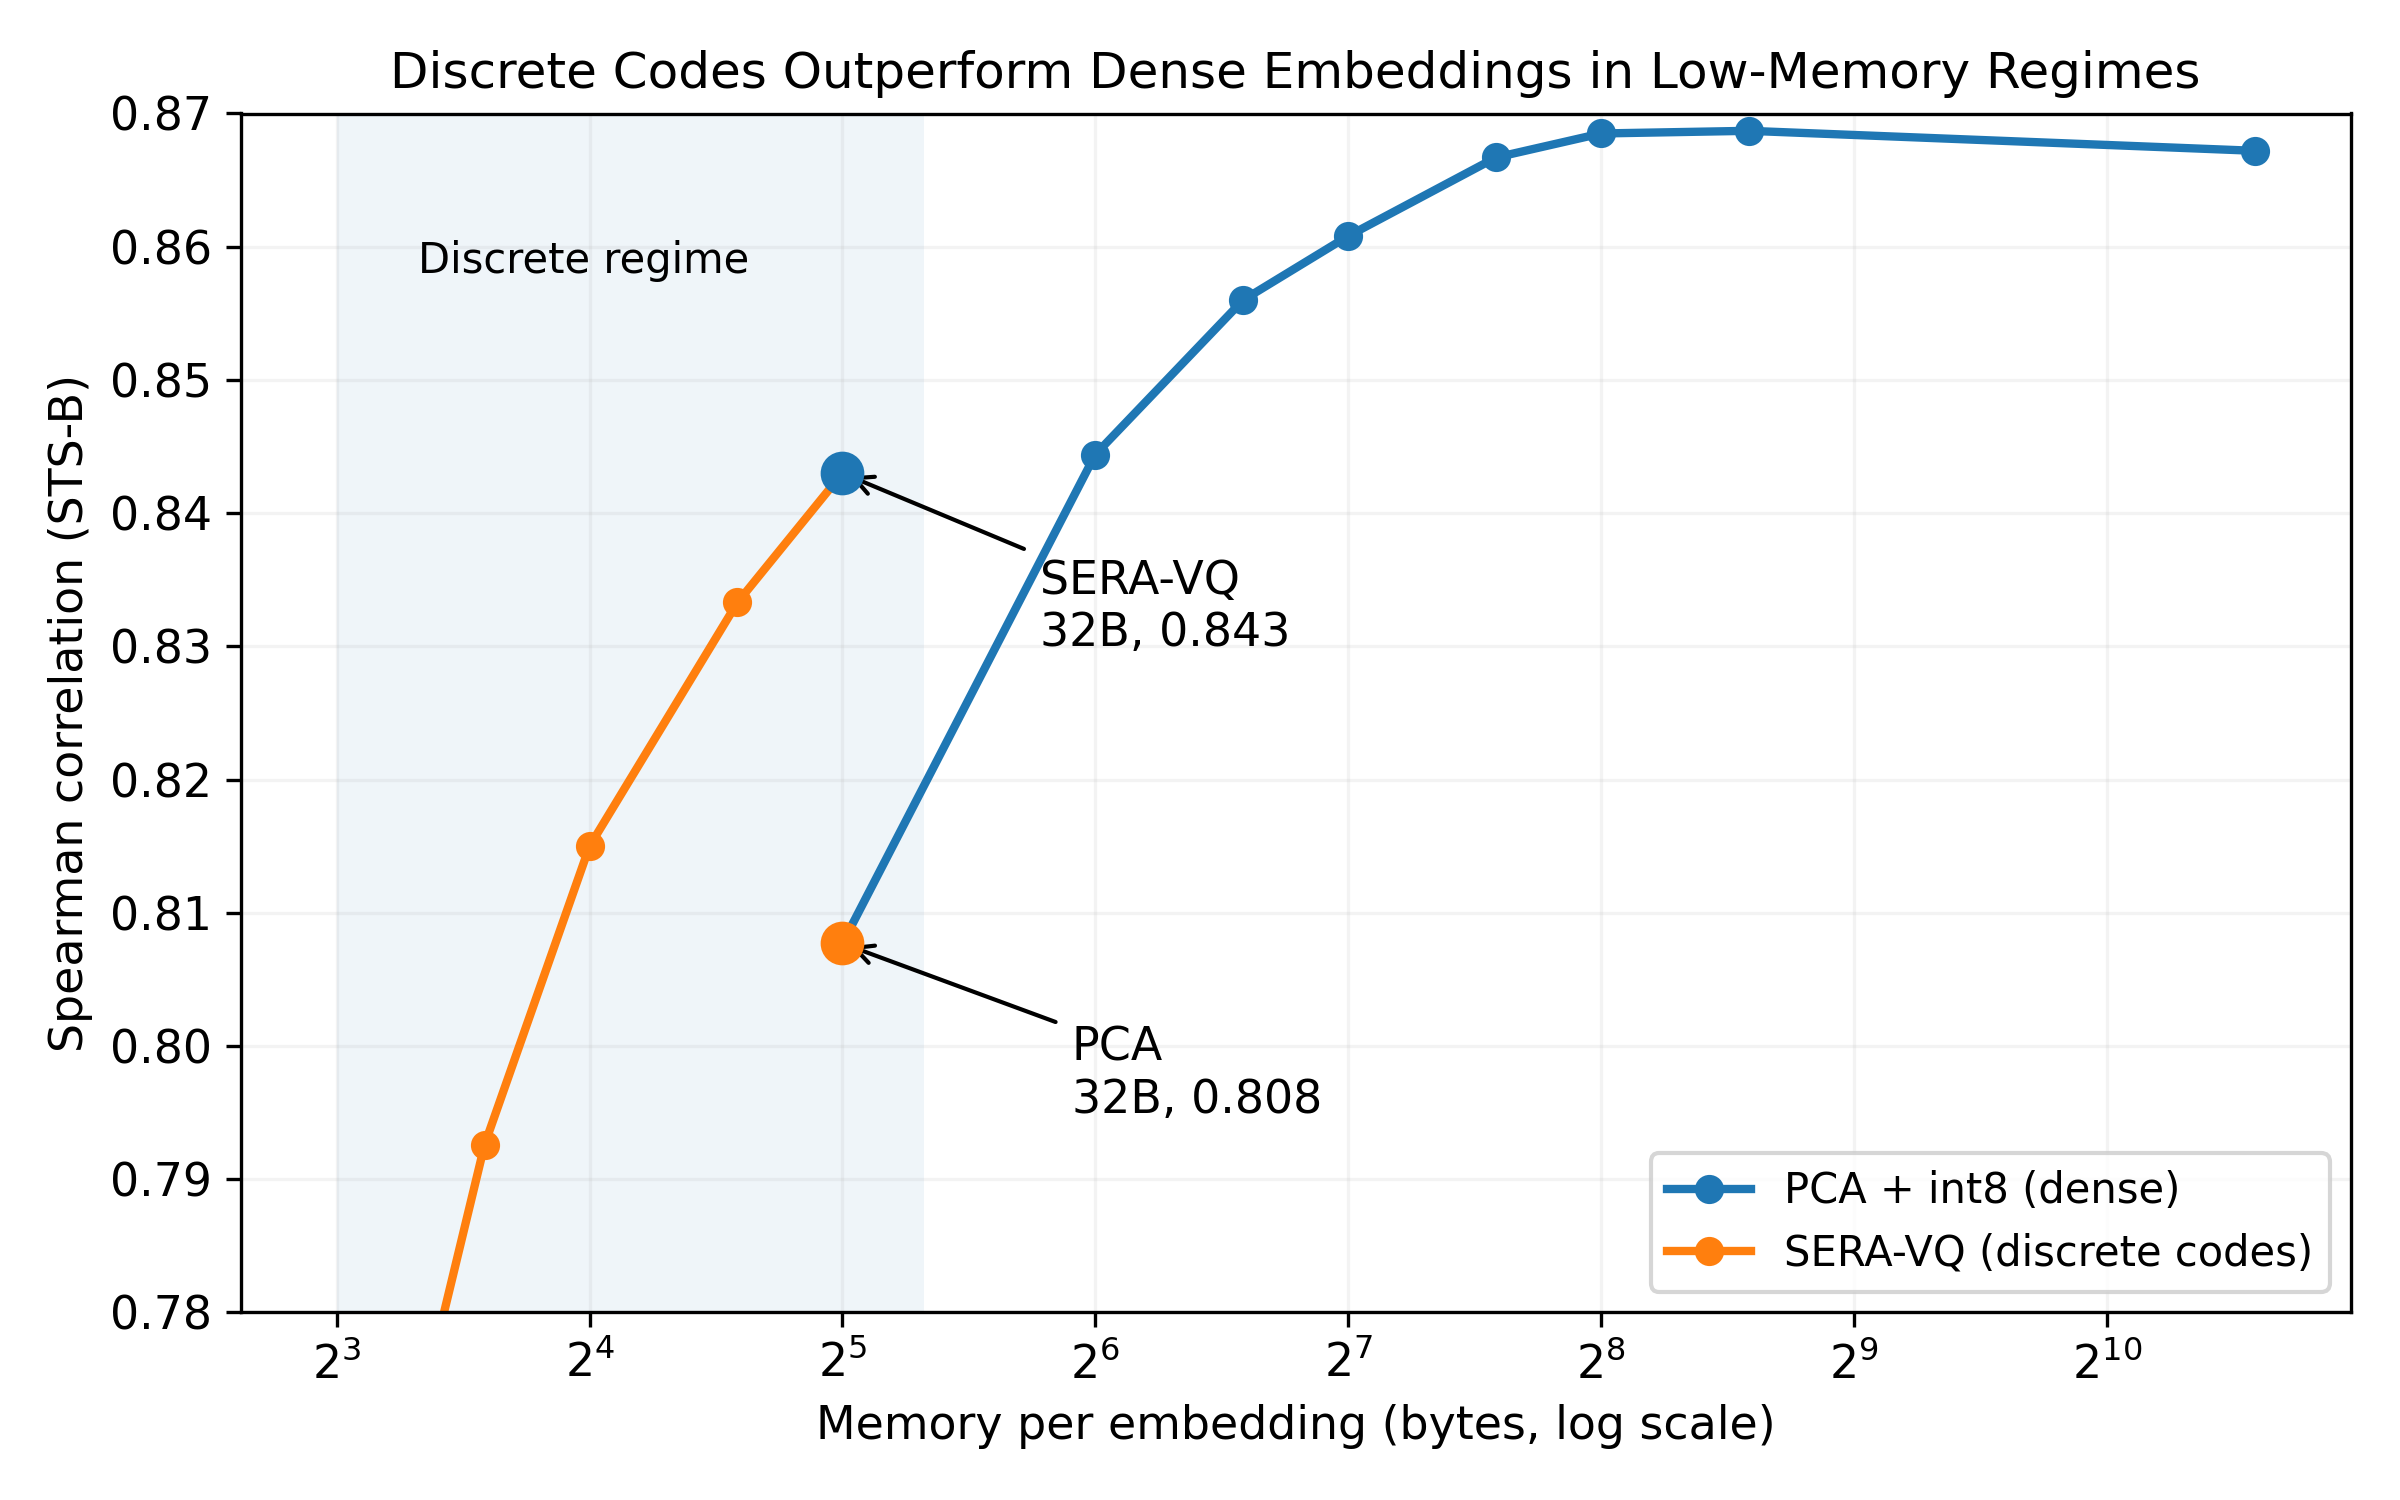
\includegraphics[width=0.9\linewidth]{figures/sera_vq_paper.png}
    \caption{Trade-off between memory and semantic similarity (STS-B). Discrete codes outperform dense PCA compression in the low-memory regime.}
    \label{fig:sts}
\end{figure}

\begin{figure}[t]
    \centering
    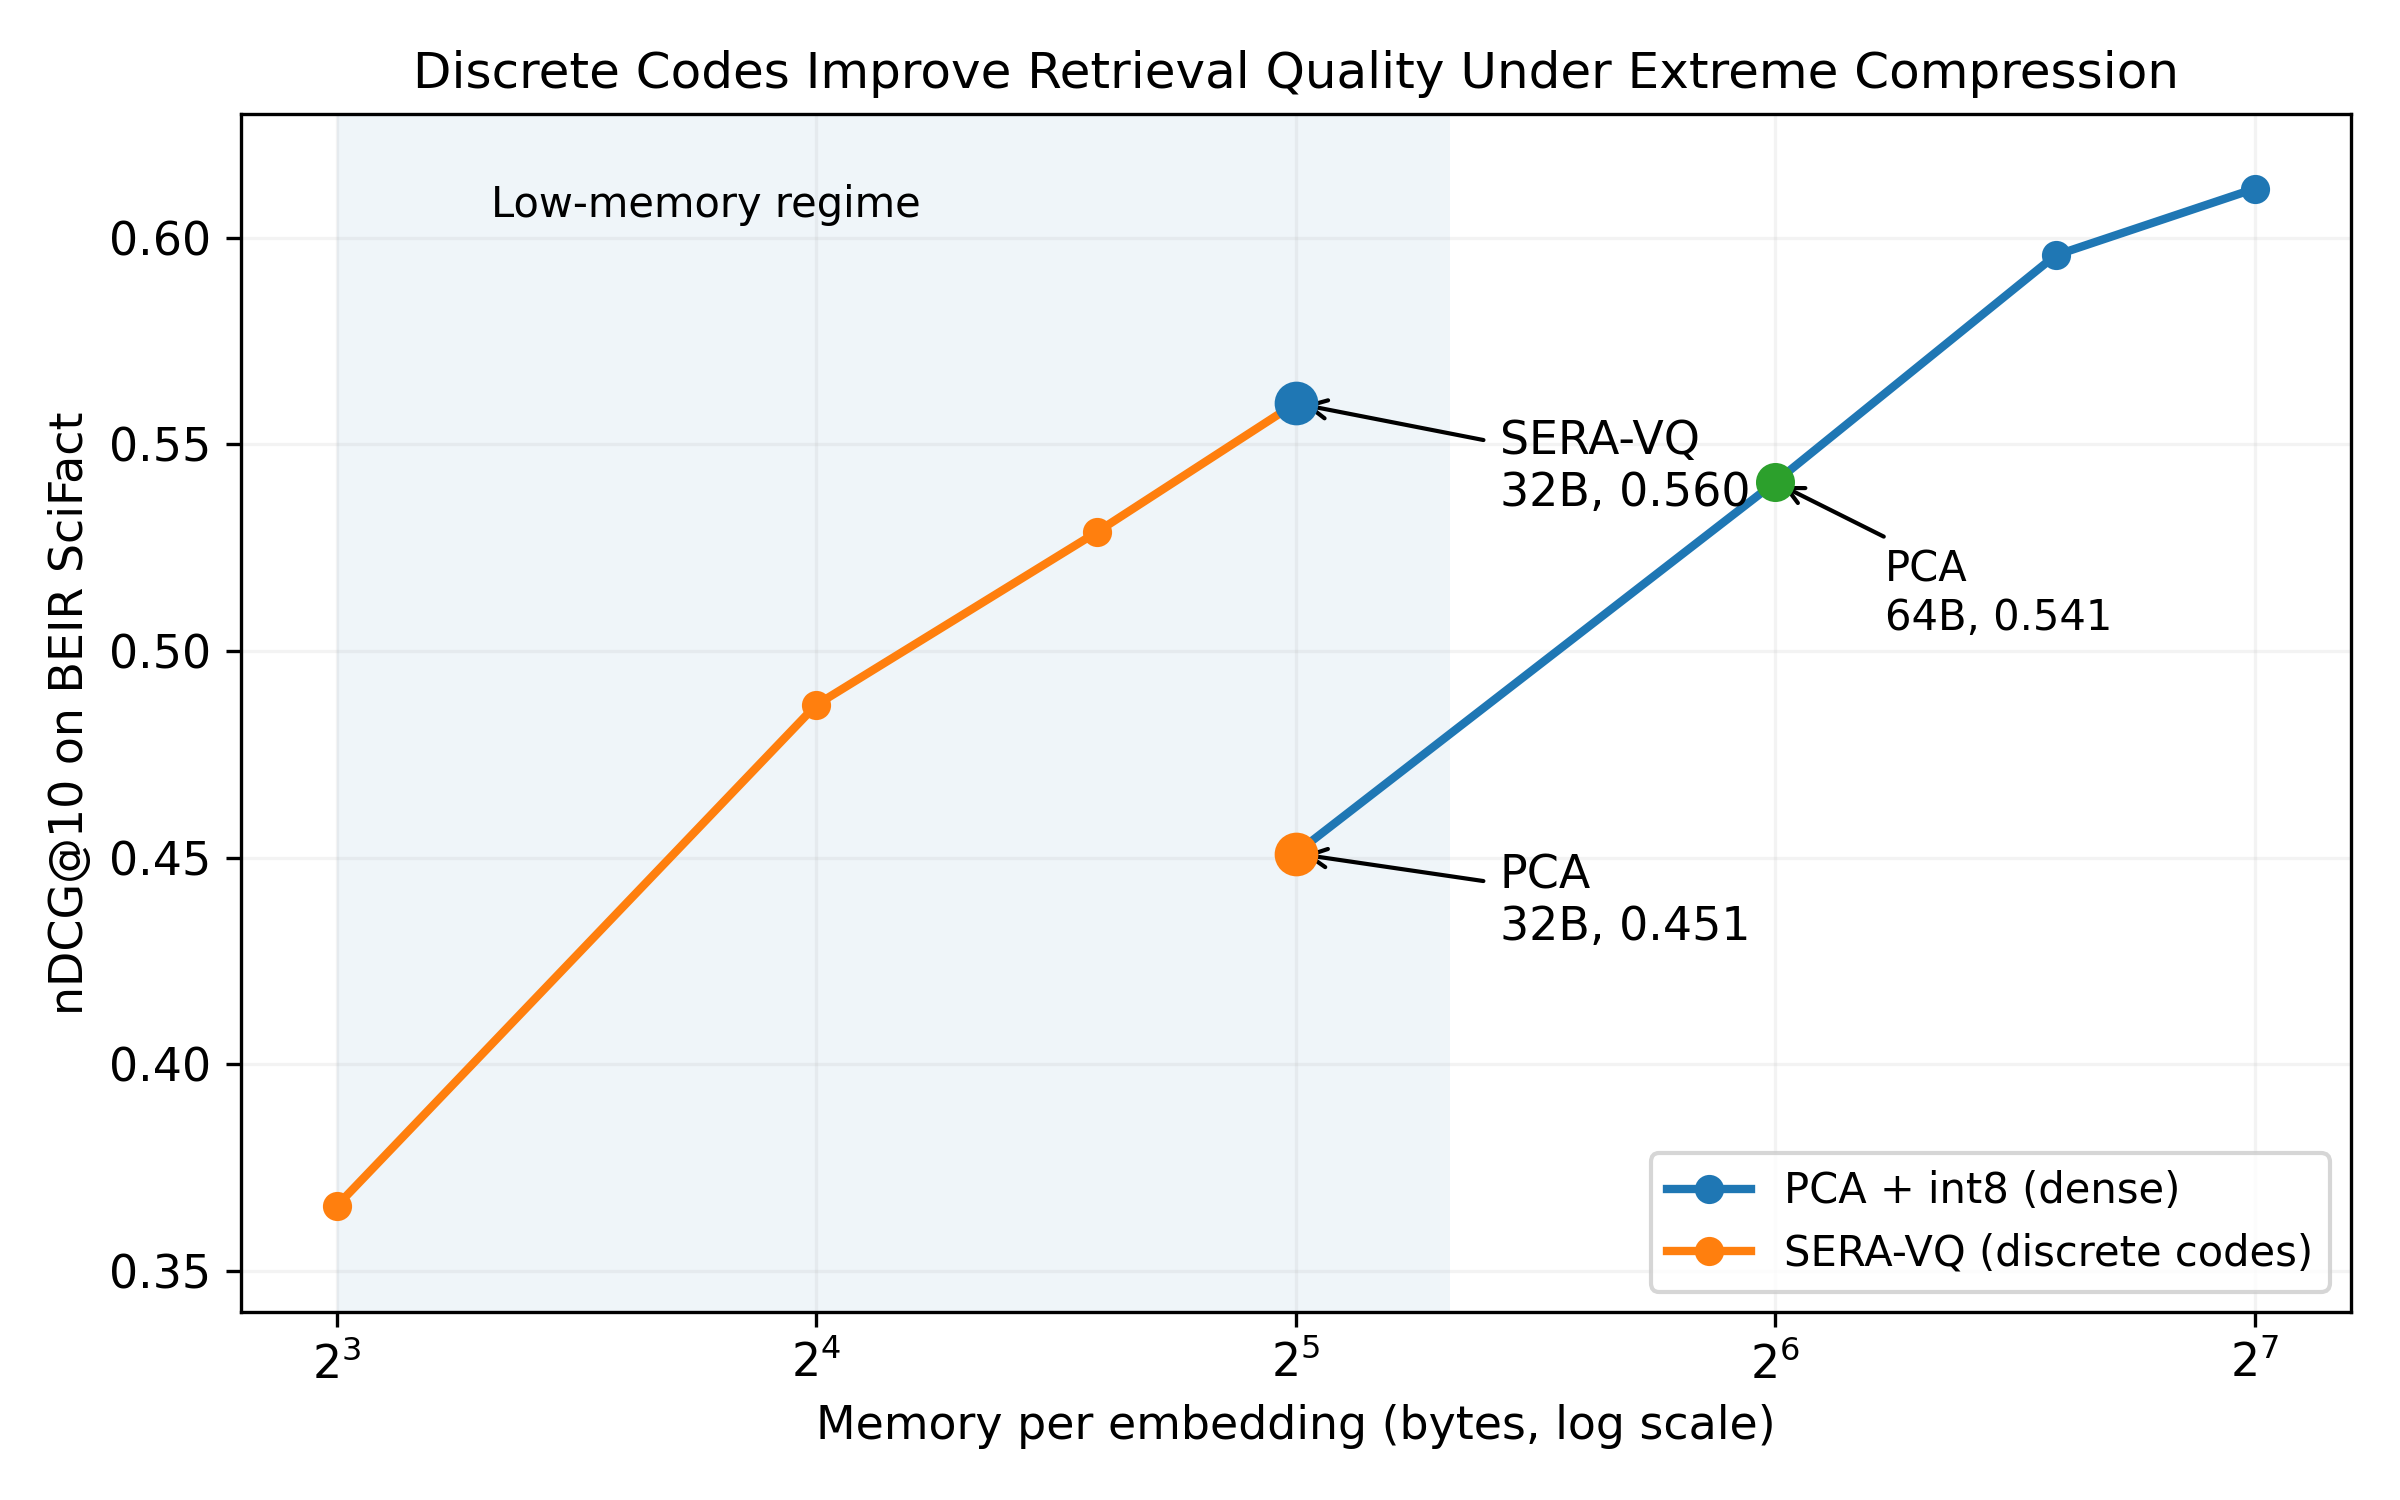
\includegraphics[width=0.9\linewidth]{figures/sera_beir_scifact_paper.png}
    \caption{Trade-off between memory and retrieval performance (BEIR SciFact). SERA-VQ significantly outperforms PCA at low memory budgets.}
    \label{fig:beir}
\end{figure}

\section{Conclusion}

In this work, we investigated the problem of embedding compression under extreme memory constraints and challenged the common assumption that dense vector representations remain optimal in this regime.

We introduced SERA-VQ, a simple pipeline combining PCA with residual vector quantization to produce compact discrete representations. Our experiments across semantic similarity (STS-B) and retrieval benchmarks (BEIR SciFact) reveal a consistent pattern: while dense PCA-based compression remains competitive at moderate to high memory budgets, discrete codes significantly outperform dense embeddings when memory is constrained to 32 bytes or less.

These results highlight the existence of a previously underexplored regime in which the optimal representation shifts from continuous vectors to discrete codes. This suggests that alternative representations should be considered when designing large-scale retrieval systems under tight resource constraints.

Overall, our findings indicate that discrete representations provide a simple, effective, and scalable alternative to dense embeddings in memory-constrained settings.

\section{Limitations and Future Work}

Our work focuses on a limited set of datasets and embedding models. While we observe consistent improvements in both STS-B and BEIR SciFact, further evaluation across a broader range of retrieval benchmarks is needed to fully validate the generality of our findings.

Additionally, our implementation reconstructs embeddings before computing similarity, which does not fully exploit the efficiency potential of discrete representations. Future work could explore direct distance computation in the compressed space using lookup tables or other techniques.

Finally, while SERA-VQ is simple and effective, more advanced quantization strategies or learned discrete representations may yield further improvements. Exploring these directions could help extend the benefits of discrete representations beyond the low-memory regime identified in this work.

\bibliographystyle{plain}
\bibliography{references}

\end{document}
